\documentclass{article}
\usepackage{graphicx}
\graphicspath{ {./images/} }

\usepackage{blindtext}
\usepackage{geometry}
\geometry{
    a4paper,
    total={170mm,257mm},
    left=25mm,
    right=25mm,
    top=15mm,
}
\usepackage{graphicx}
\usepackage{amsmath,amsthm,amssymb}
\usepackage{nccmath}
\usepackage{mathtext}
\usepackage[T1,T2A]{fontenc}
\usepackage[utf8]{inputenc}
\usepackage[french, russian]{babel}

\setlength{\parindent}{0mm}

\title{
\textit{\small{Georgii Potoshin, 2023, малый мехмат}}\\
\vspace{0.3ex}
\textit{\huge{Découpage}}\vspace{1ex}
}

\date{\vspace{-8ex}}

\begin{document}
\maketitle

\begin{center}\textsc{\Large{Exercices pour la discussion}}\end{center}
\begin{enumerate}
    \item Découper le carré en \textbf{a)} 4 ; \textbf{b)} 9 ; \textbf{b)} 17 carrés.
    \item Quatre nains ont hérité d'un verger de leur oncle, délimité par 16 allumettes, avec 12 arbres fruitiers. L'emplacement des arbres est indiqué sur le dessin. Divisez le jardin en utilisant 12 allumettes en quatre parties égales contenant chacune un nombre égal d'arbres (les parties égales doivent avoir la même forme et la même taille).
    \vspace{-3ex}
    \begin{center}
        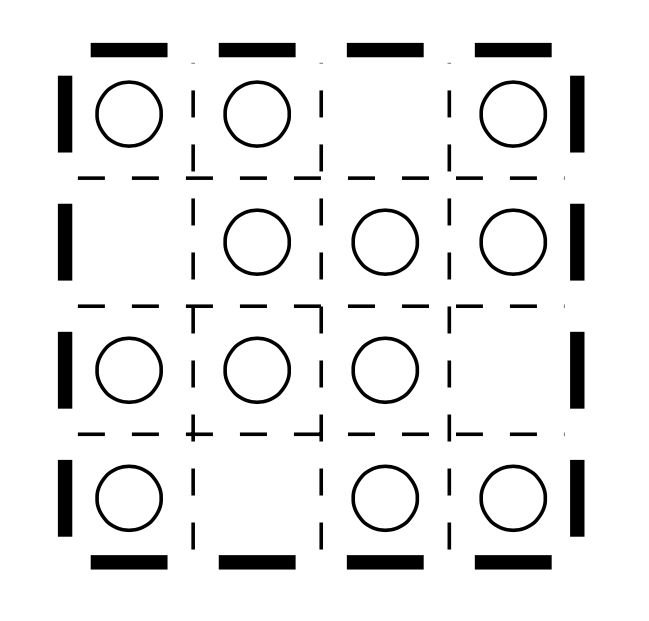
\includegraphics[scale=0.1]{2.png}        
    \end{center}
    \vspace{-3ex}
    \item La pastèque a été coupée en quatre et consommée. Il en est ressorti cinq croûtes. Comment cela se fait-il ?
    \item Découpez la figure représentée sur le dessin en quatre parties égales.
    \vspace{-2.2ex}
    \begin{center}
        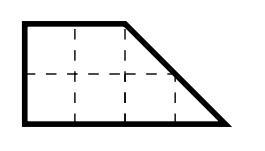
\includegraphics[scale=0.2]{4.png}        
    \end{center}
    \vspace{-3ex}
    \item Plier la serviette carrée en deux, puis plier à nouveau le rectangle en deux. Le carré a été coupé avec des ciseaux en ligne droite. La serviette peut-elle être divisée en \textbf{a)} 2 morceaux ; \textbf{b)} 3 morceaux ; \textbf{c)} 4 morceaux ; \textbf{d)} 5 morceaux ?
    \item Divisez la figure affichée en quatre parties identiques de manière à ce qu'elles puissent être assemblées pour former un carré 6 × 6. Assurez-vous que le carré résultant présente une coloration en damier.
    \vspace{-2ex}
    \begin{center}
        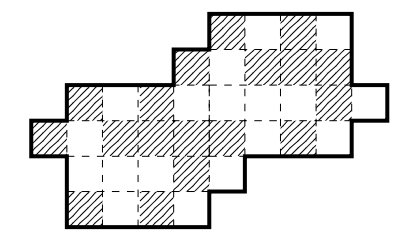
\includegraphics[scale=0.3]{6.png}        
    \end{center}
    \vspace{-3ex}
\end{enumerate}

\vspace{1ex}
\begin{center}\textsc{\Large{Devoirs}}\end{center}
\begin{enumerate}
    \item \textbf{a)} Divisez un rectangle de dimensions 4 × 9 en deux morceaux de manière à ce qu'ils puissent être assemblés pour former un carré de dimensions 6 × 6. \par
    \textbf{b)} Divisez un rectangle de dimensions 9 × 16 en deux morceaux qui peuvent être pliés de manière à former un carré.
    \item Découpez chacune des formes suivantes en deux morceaux identiques.
    \vspace{-2ex}
    \begin{center}
        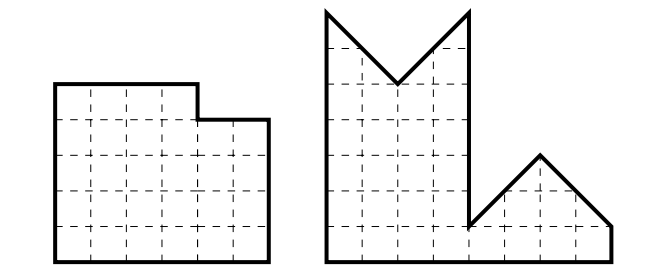
\includegraphics[scale=0.3]{8.png}        
    \end{center}
    \vspace{-3ex}
\end{enumerate}
\end{document}
